\chapter{Diboson studies}
\label{chap:dibosons}

The resonant diboson processes $\Z\Z$ and $\W\Z$ are an irreducible background of the
dark matter searches involving any Z boson in the final state.
In final states with little hadronic activity e.g. this work, 
the other background processes which contribute substantially are easy to reject and pare down.
Then, the diboson becomes the main problem due to our limited theoretical understanding, and nothing beside remains.

Below, I survey the current status of theoretical calculations for dibosons. 
Then, I discuss a strategy which makes use of independent control samples from the experimental data,
to improve upon inaccuracies arising from those calculations.

\section{Limitations of simulating diboson processes}

All simulated physics processes in this work are susceptible to uncertainties due to: the proton parton distribution functions; the QCD scale, $\alpha_s$; and the renormalization and factorization scales in the quantum field theory.
Consistent with the other processes, these effects are propagated to both the overall cross sections and the transverse momentum spectra of the $\Z\Z$ and $\W\Z$ processes.
The details of this propagation are described later, in section ??.
For the purposes of motivating this chapter, it suffices to say that the effect of these is roughly 10\%. 

Meanwhile, as previously outlined in \ref{sec:higher-order-corrections}, the endgame-level precision for the $\Z\Z$ and $\W\Z$ simulations is NNLO in QCD and NLO in electroweak.
Since no cohesive theoretical calculation is available at this level of precision, our duct-tape assembly of higher-order corrections come at a price.
Namely, we do not count the contribution from diagrams at NLO in both QCD and electroweak. Thus arises the so-called "QCD-electroweak cross-term."

The overall electroweak NLO correction to the $\W\Z$ process is relatively small, since the virtual corrections and photon-induced corrections partially cancel.
Therefore, the NLO QCD-electroweak cross-term for the $\W\Z$ process is also small.
On the other hand, the electroweak NLO corrections to the $\Z\Z$ process are large and momentum-dependent.
They bring a 10\% net reduction of the overall $\Z\Z$ yield, with a strong dependence on the lesser boson $p_T$.
The $\met$ spectrum becomes much softer, with a correction of around $-40\%$ at lesser Z boson $p_T$ of $700 \GeV$.
For this reason, we cannot neglect the QCD-electroweak cross term for the $\Z\Z$ process, and a conservative
assessment of this missing term gives an overall effect of roughly $25\%$.

Yet another conservative step is taken regarding the NNLO QCD corrections.
For lack of a better method, we carry forward the PDF and QCD scale uncertainties from the original POWHEG calculation at NLO in QCD,
even though the final distributions are corrected to NNLO in QCD.
This represents another setback in our understanding of the diboson processes.

So far, in this chapter I have presented a bleak picture of the diboson calculations.
There is a silver lining to this: it is possible to control these cumbersome uncertainties by exploring the experimental data.
The name of the game is to extrapolate from diboson events with fully visible decays, to the transverse momentum spectrum of diboson processes with substantial missing energy. 
The sections below outline the statistically independent control samples, in which are gathered these aforementioned visible diboson decays.

\section{Three-lepton control sample}
\label{sec:wz3l}
The $\WZ$ process is estimated from events with three well-reconstructed leptons and a nominal amount of $\met$.

Events must have exactly two opposite-charged electrons/muons with $\pt > 25/20~\GeV$ each.
The mass of this dilepton system ($\mll$) is required to be $\left|\mll-m_{\Z}\right| < 15\GeV$, consistent with the decay of a $\Z$ boson.
An additional well-identified electron or muon is required, representing the W boson.
To enhance the purity of the $\WZ$ selection, $\met$ of at least 30\GeV is required,
the invariant mass of all three leptons $m_{3\Lep}$ is required to be larger than $100\GeV$,
and the invariant mass between all opposite sign-same flavour lepton pairs ($m_{2\Lep}$) is required to be larger than $4\GeV$.
These requirements follow the procedure used in the CMS measurement of the $\WZ$ production cross-section~\cite{Khachatryan:2016tgp}.

Since there is no danger of contamination, no veto on additional hadronically-decaying $\tau$ leptons is applied.
A relaxed b-jet veto is applied which rejects events where a jet passes the most stringent b-jet identification requirement.

\section{Four-lepton control sample}
\label{sec:zz4l}
The $\ZZ$ process is estimated from events with four well-reconstructed leptons.
In addition to a stringently-identified $\Z$ candidate as in Section~\ref{sec:wz3l}, 
a second candidate is required, whose decay products only need to pass loose identification requirement.
This choice reflects the very high purity of the four-lepton selection. 
For both candidates, the $\Z$ mass requirement is enforced.

Again as in Section~\ref{sec:wz3l}, there is no hadronic $\tau$ veto, and a relaxed b-jet veto is applied.

\section{Emulation of the missing energy}
\label{sec:fakemet}
We now seek to solve the aforementioned problem. 
Using the pure control samples with three or four leptons, the aim is to extrapolate
to an estimation of the missing energy spectra for $\Z\Z$ and $\W\Z$ events 
with only two reconstructed leptons and missing energy in the final state.
The $\W\Z$ process can appear this way due to a lost lepton.
A lepton can be lost due to inefficiency in the reconstruction and identification of leptons, or otherwise the limited detector acceptance.

We extrapolate to the $2\ell+\met$ final state by furnishing a quantity known as the emulated $\met$ or so-called ``fake $\met$.''
For the $\WZ$ process, the fake $\met$ is the true $\W$ boson $\pt$.
It is estimated by calculating the vectorial sum of the $\met$ vector and the transverse momentum vector of the third lepton.
For the $\Z\Z$ process, the fake $\met$ comes from taking the sum of any nominal true $\met$ and one of the leptonically-decaying $\Z$ bosons.
The $\Z$ boson which is made to vanish in this disappearing act is chosen to be the one whose reconstructed invariant mass is further from the
nominal $\Z$ mass of $91.1876 \GeV$.
\footnote{The choice of which $\Z$ candidate to use for the emulation of the $\met$ is arbitrary and has almost no effect on the resulting distribution.}.

The resulting emulated \met spectra are shown in Fig.~\ref{fig:histo_fakemet}.

\begin{figure}[htbp]
\centering
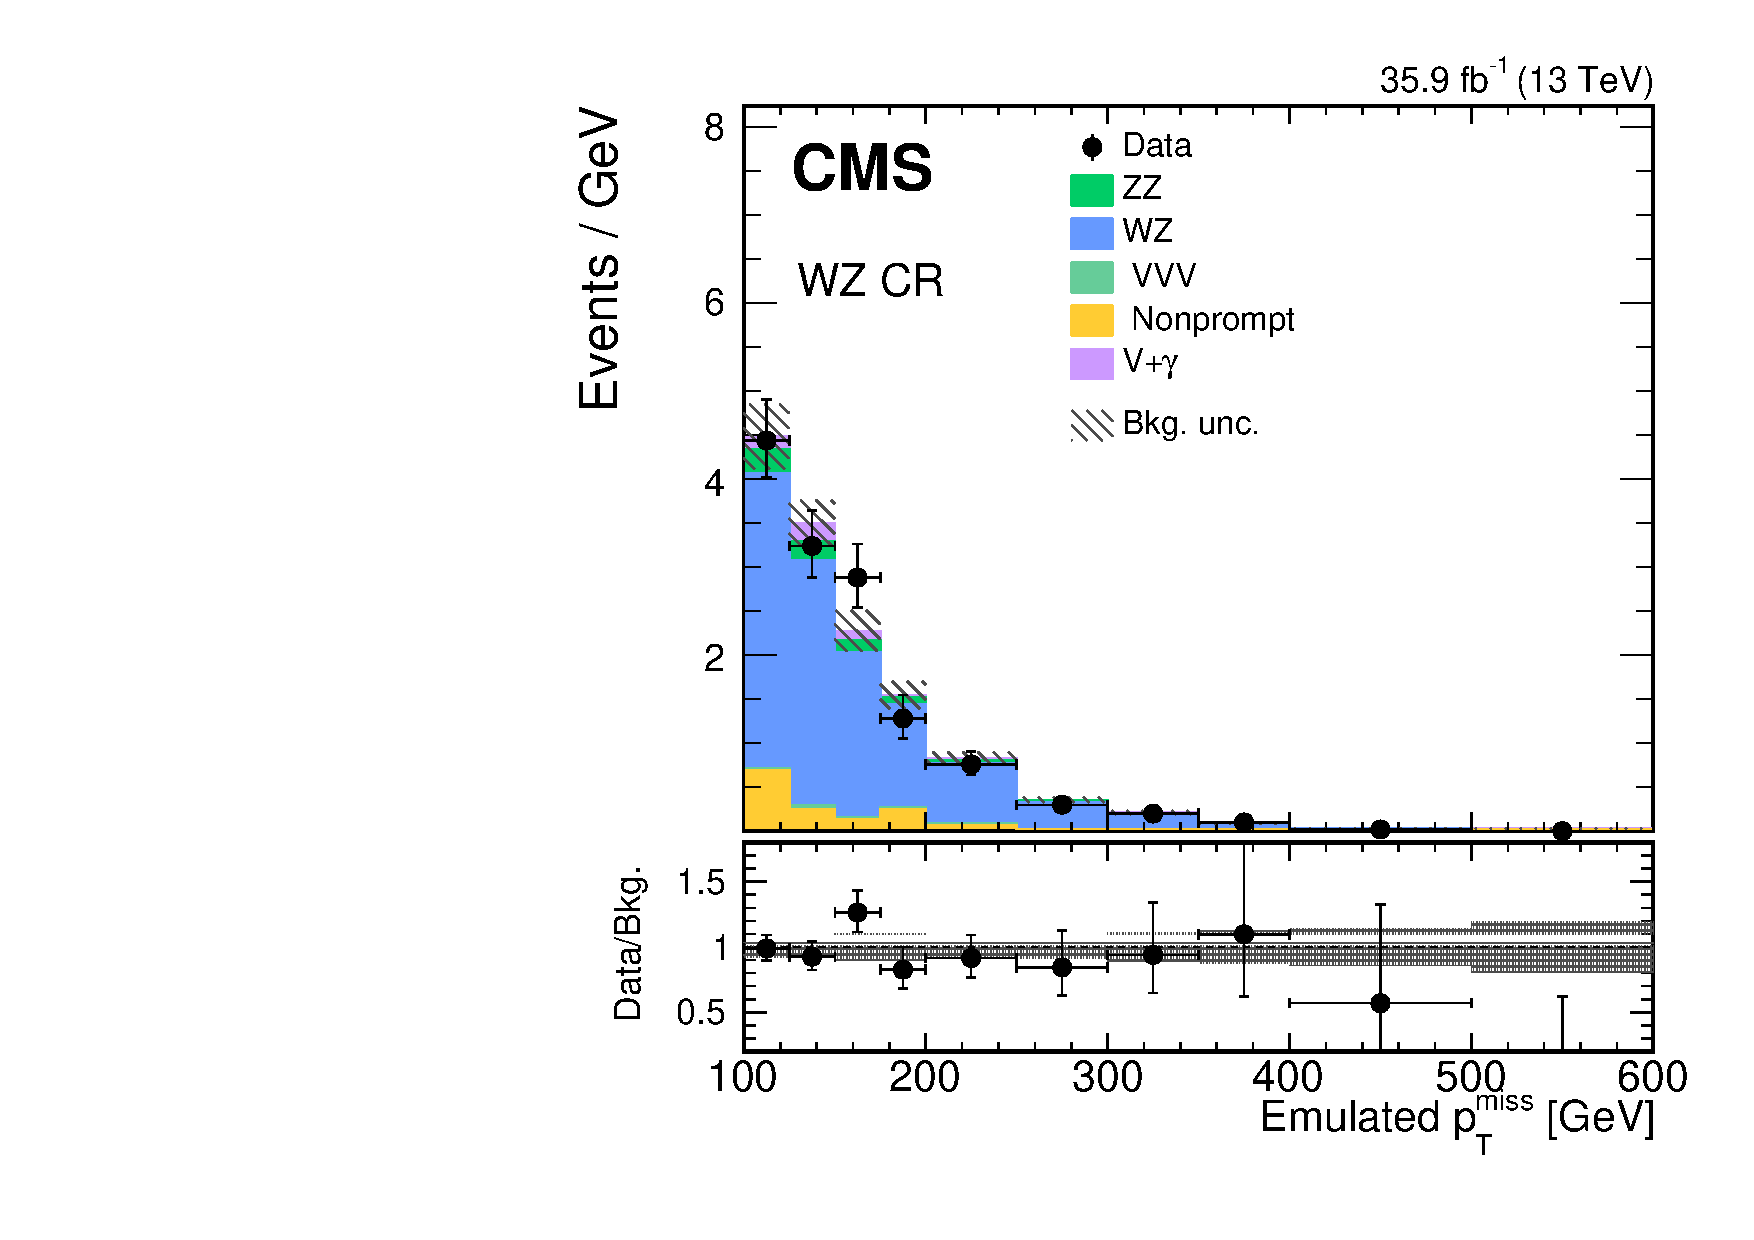
\includegraphics[width=0.48\textwidth]{figures/wz_fakemet_allcuts_postfit.pdf}
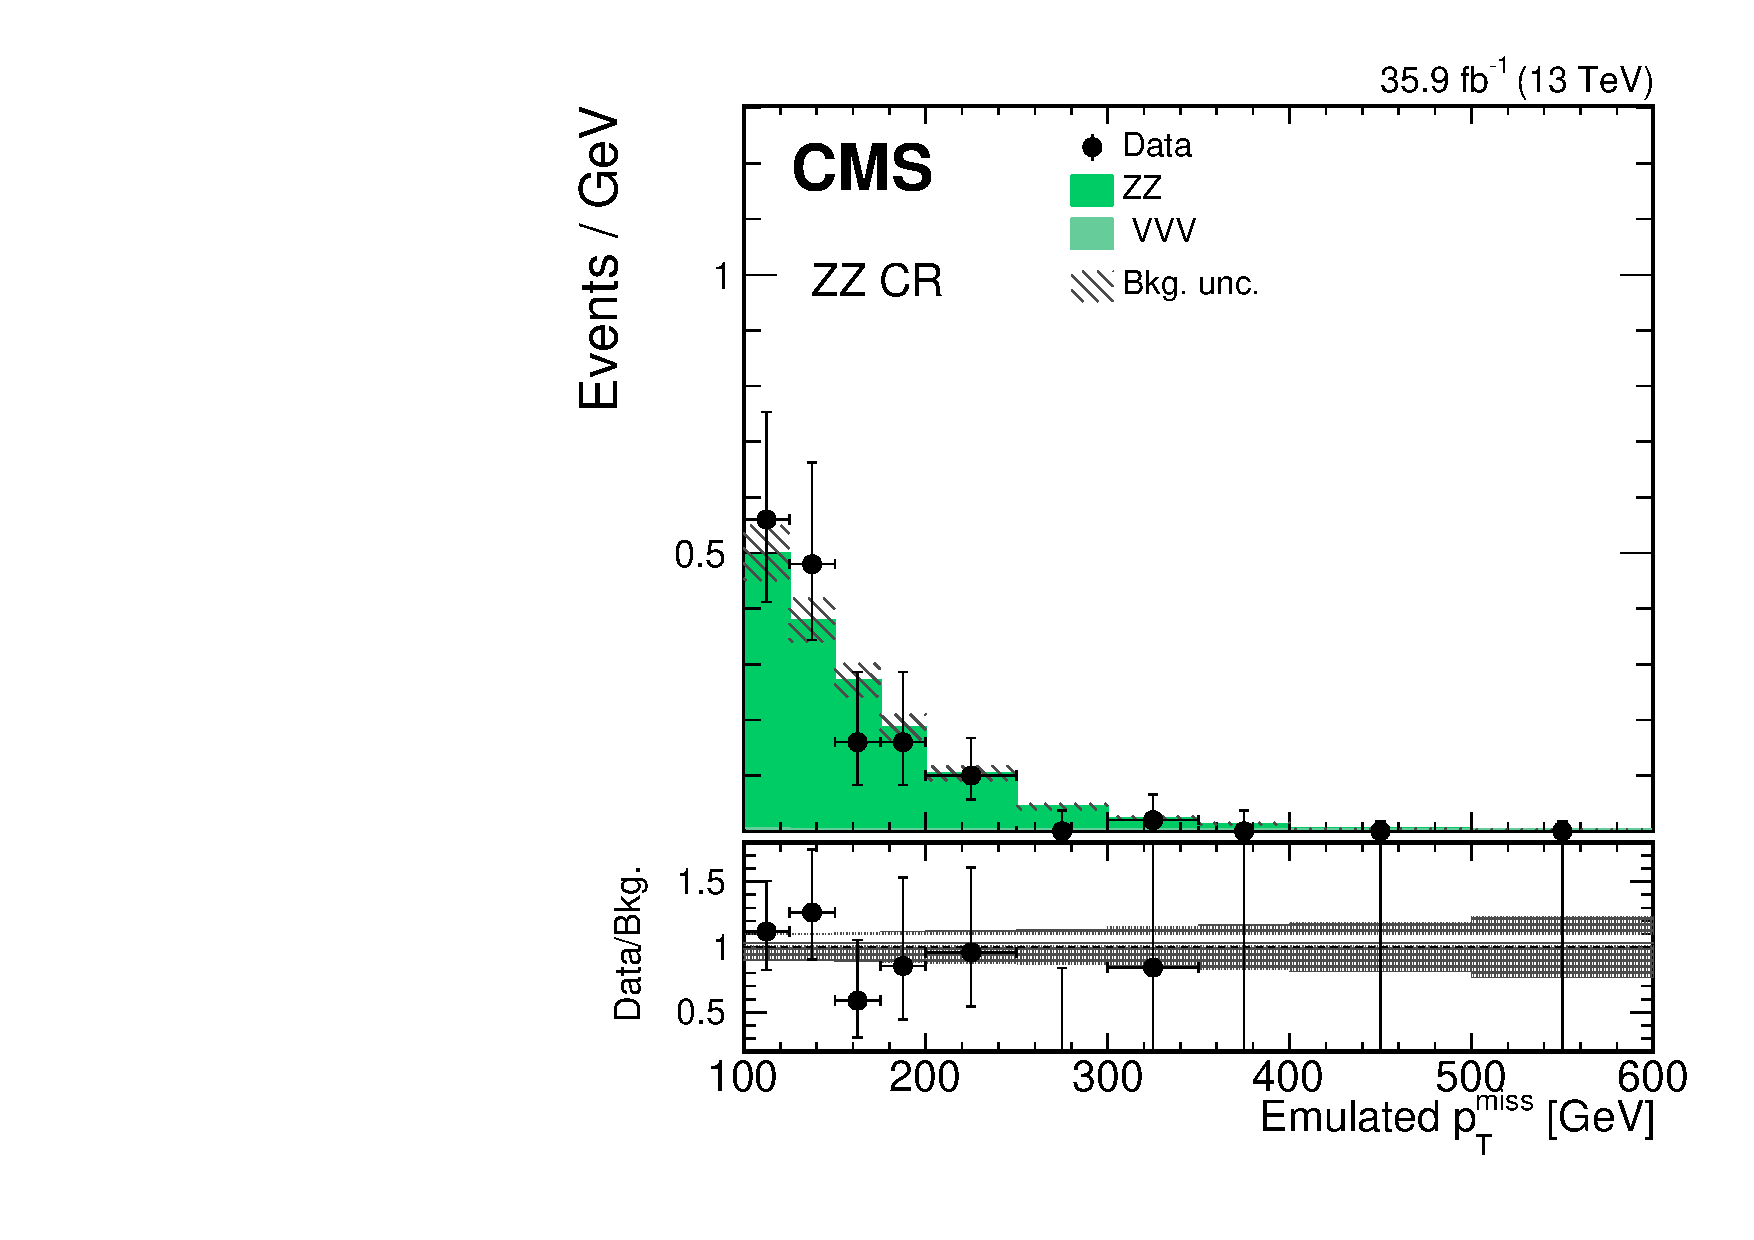
\includegraphics[width=0.48\textwidth]{figures/zz_fakemet_allcuts_postfit.pdf}
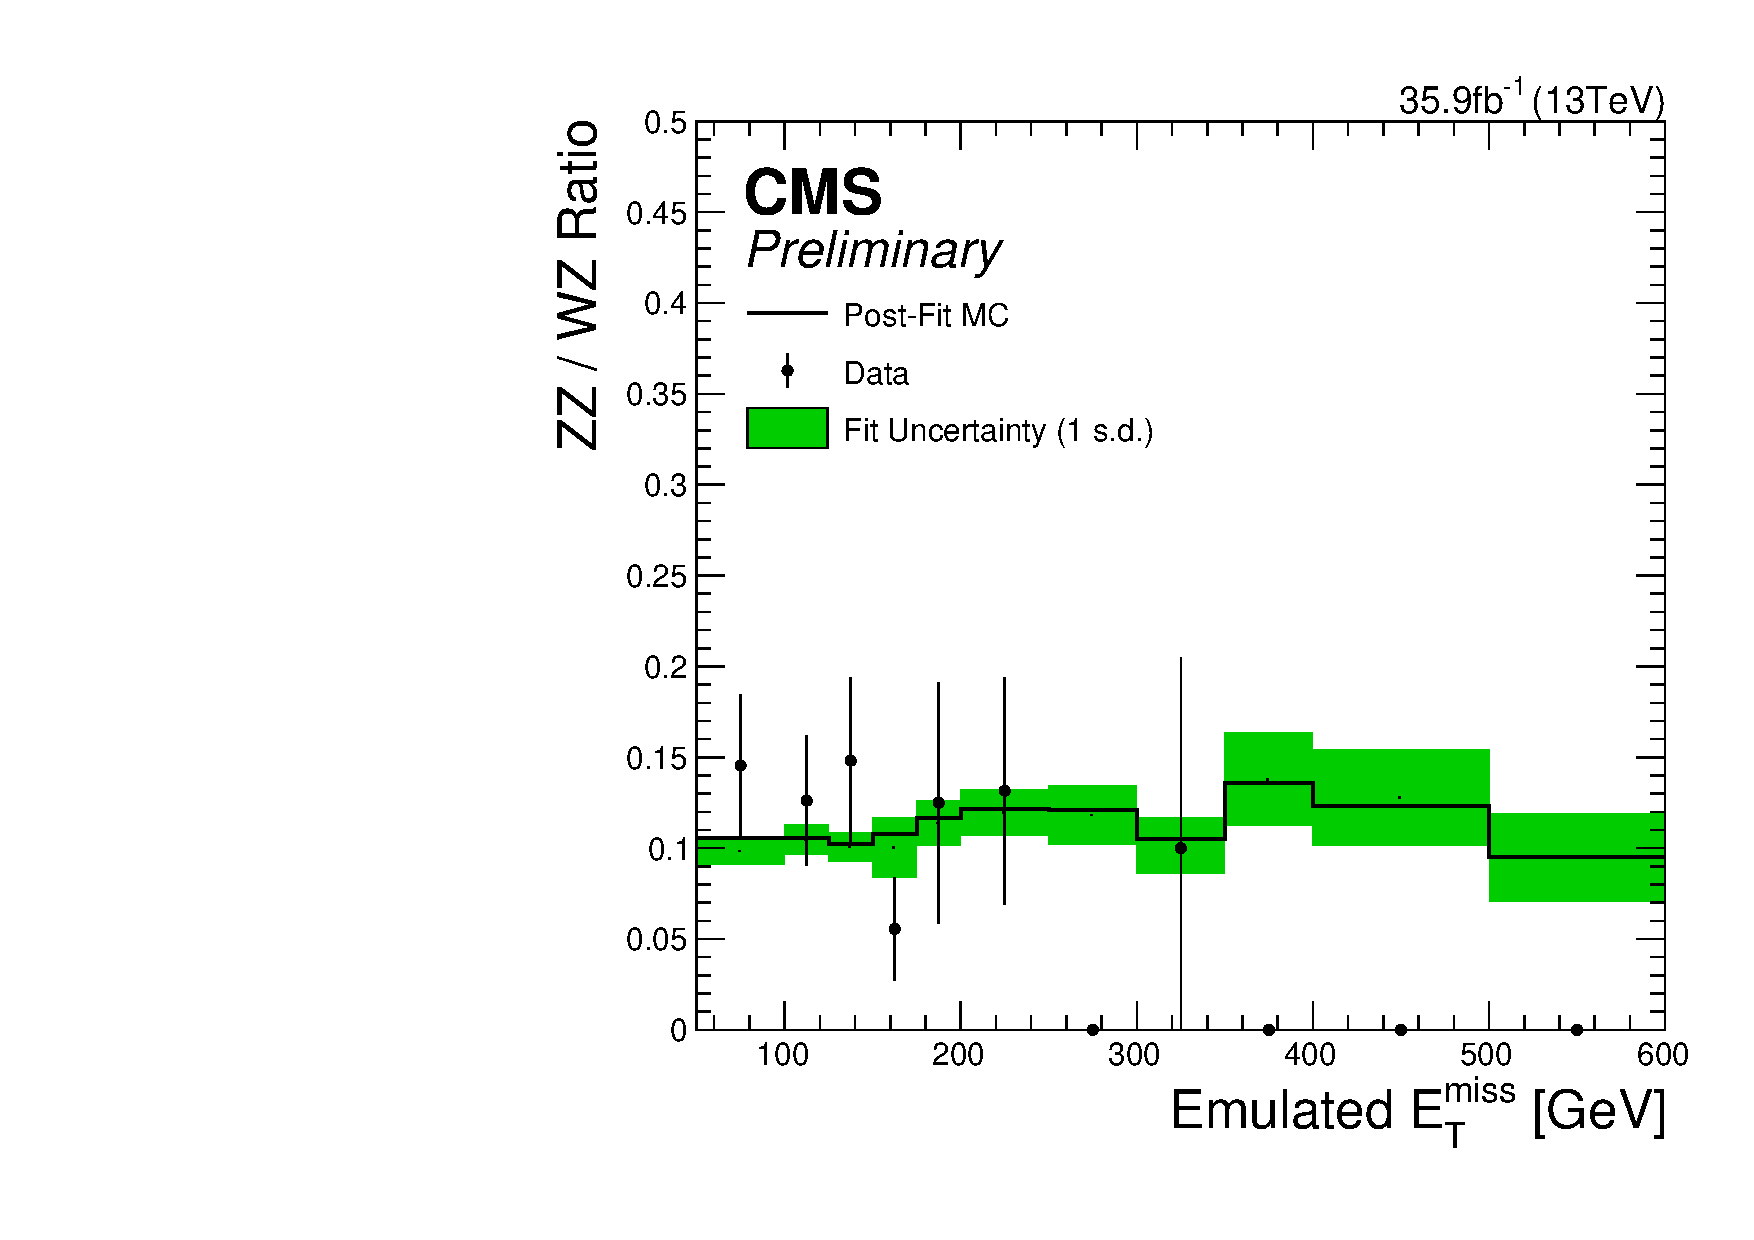
\includegraphics[width=0.48\textwidth]{figures/ratio_zzvswz.pdf}
\caption{Emulated $\met$
distribution for  the $\W\Z \to 3\Lep\nu$(top left) and $\Z\Z \to 4\Lep$ (top right)
control regions, and the ratio between both distributions in data and simulation (bottom).
 Uncertainty bands correspond to both statistical and systematic uncertainty.}
\label{fig:histo_fakemet}
\end{figure}


